\cohead{\Large\textbf{Eigenschaften von \(\sin x /\cos x\)}}
\fakesubsection{Eigenschaften der Sinus- und Cosinusfunktion}
\begin{minipage}{\textwidth}
	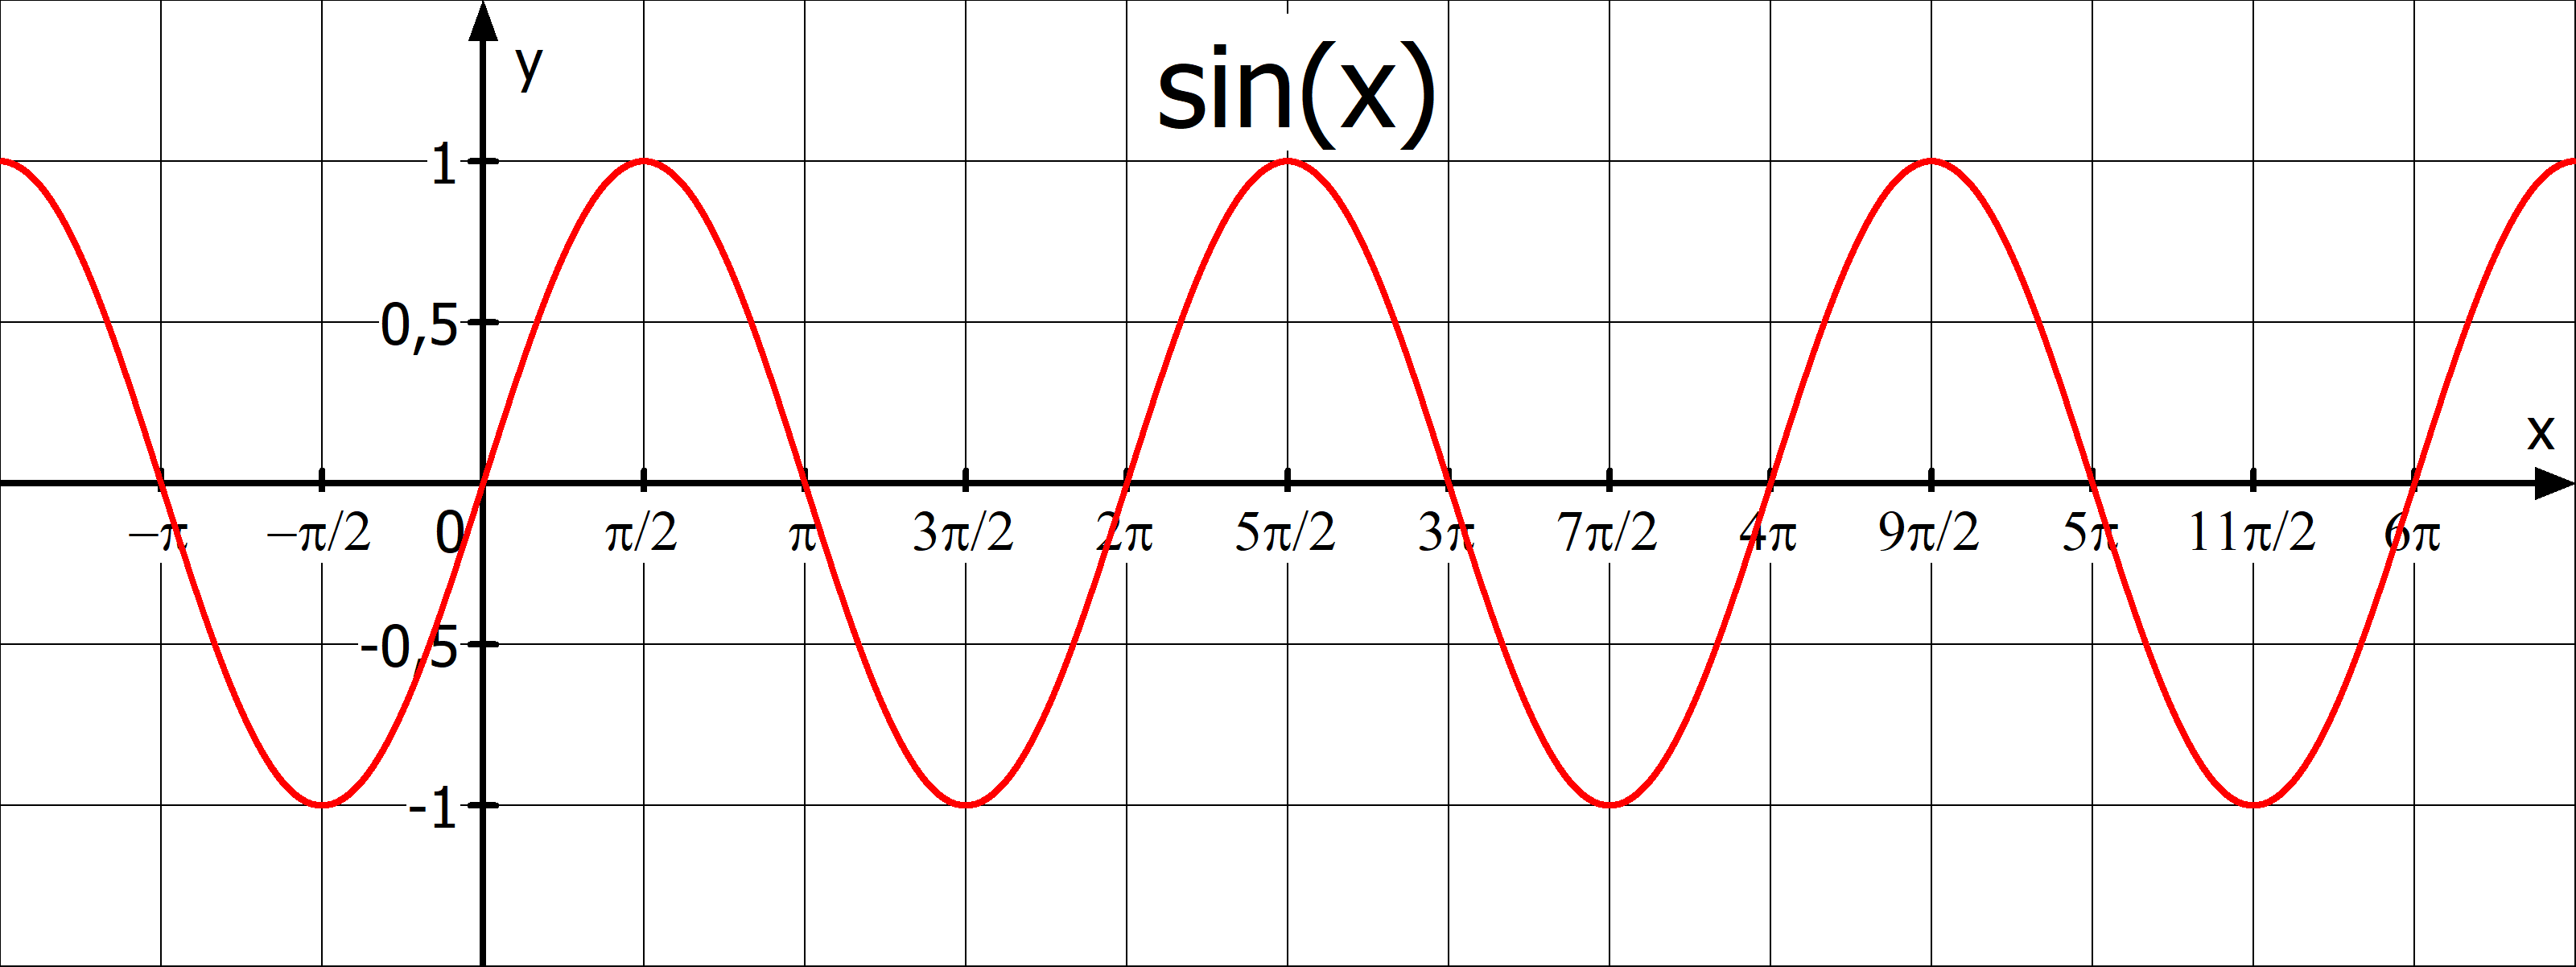
\includegraphics[width=\linewidth]{\trigonometrie/pics/sinx.png}
\end{minipage}%

\bigskip

\begin{minipage}{\textwidth}
	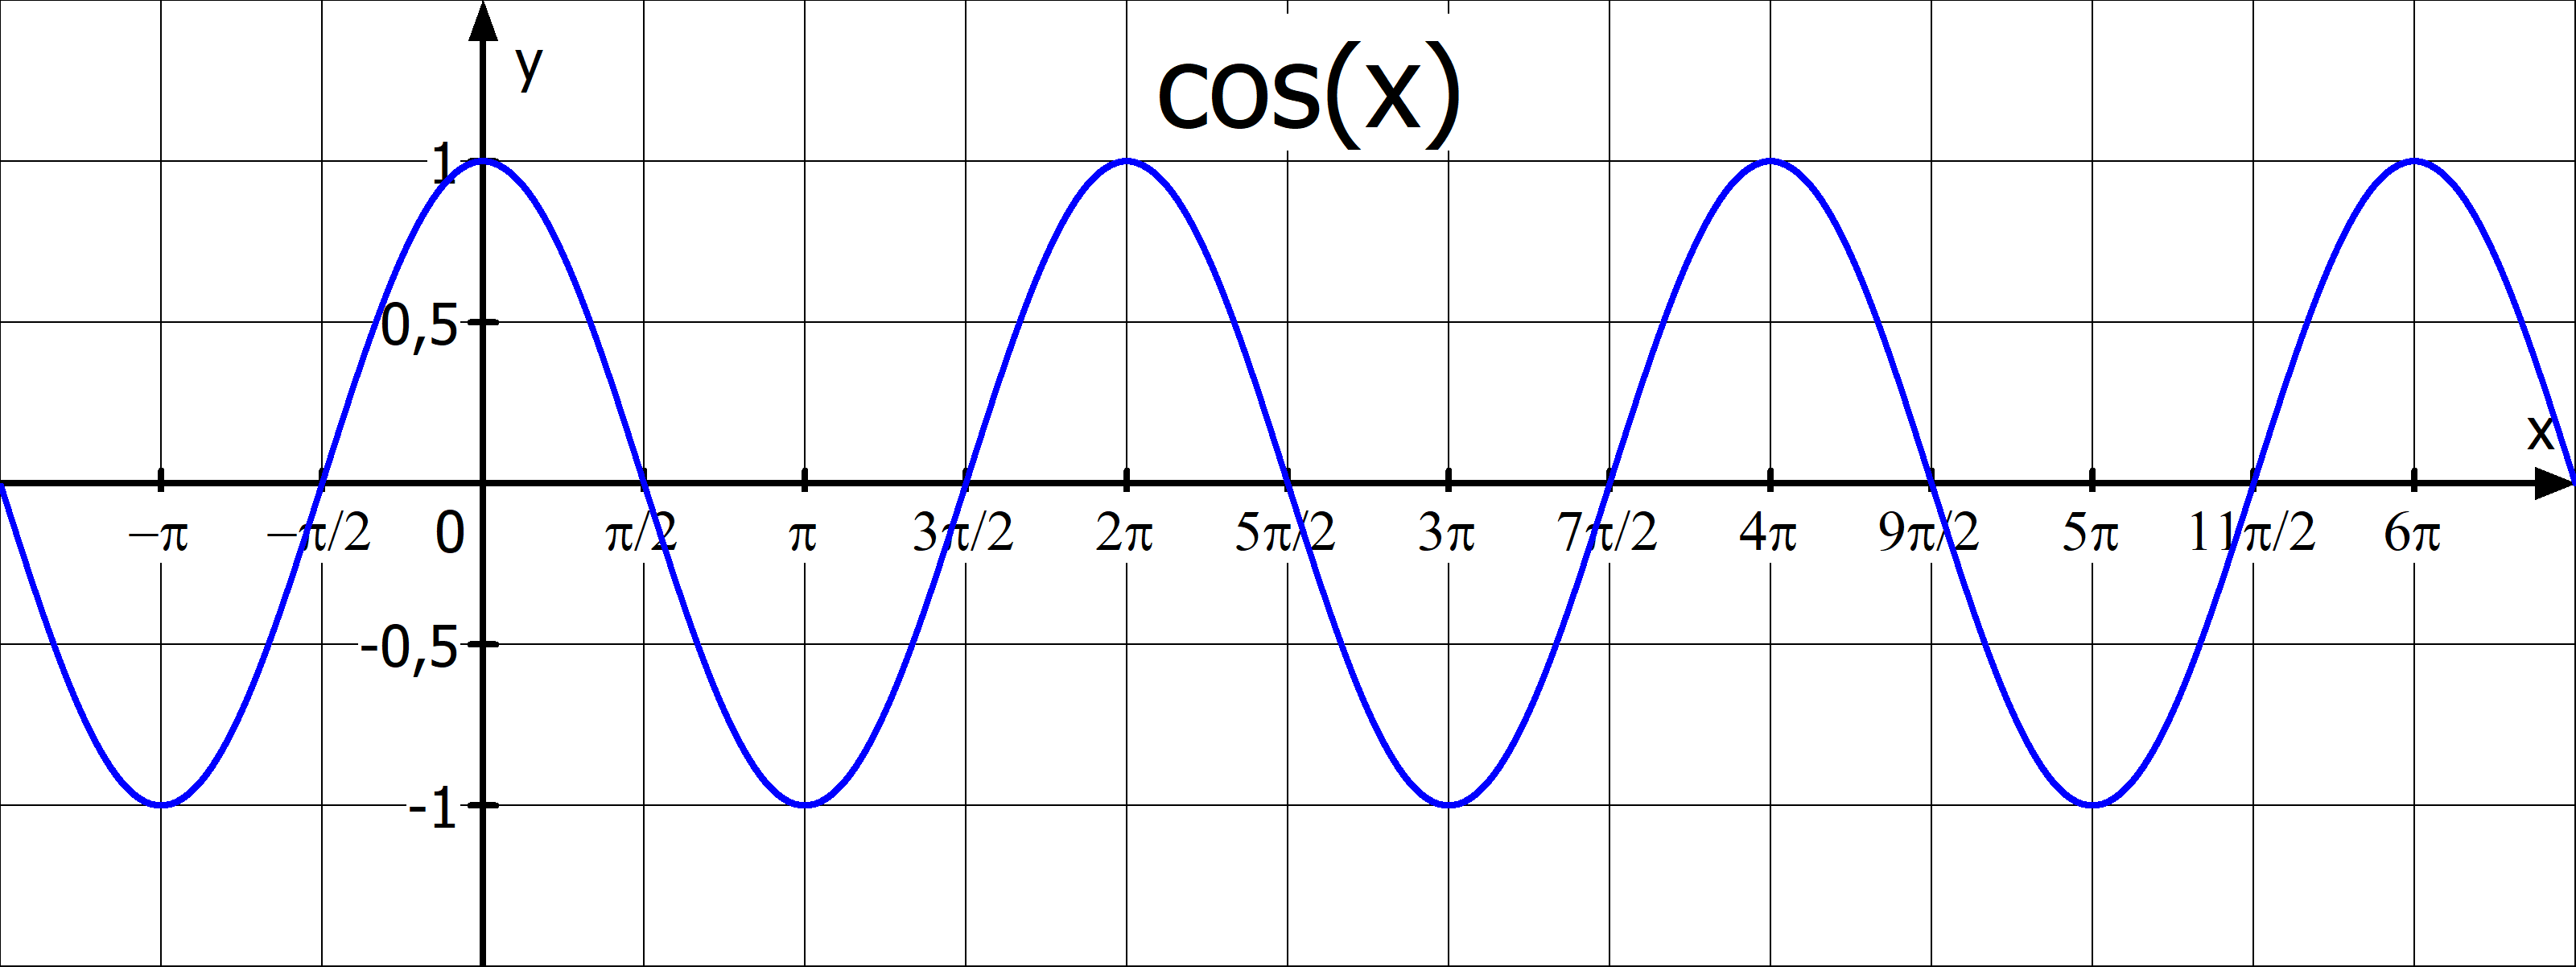
\includegraphics[width=\linewidth]{\trigonometrie/pics/cosx.png}
\end{minipage}%

\bigskip

Folgende Begriffe/Eigenschaften benötigen wir:
\begin{itemize}
	\item Periode \(p\):

	\textcolor{loes}{Die Länge des kleinstmöglichen Ausschnitts, nach dem sich das Schaubild der Funktion wiederholt. Für beide Funktionen ist \(p=2\pi\).}

    \vspace{\baselineskip*\real{2}}

	\item Mittelwert \(d\):

	\textcolor{loes}{Der \(y\)-Wert um den das Schaubild hin- und herpendelt. Für beide Funktionen ist \(d=0\).}

    \vspace{\baselineskip*\real{3}}

	\item Amplitude \(a\):

	\textcolor{loes}{Der maximale Abstand der Funktionswerte vom Mittelwert. Die Amplitude ist immer positiv. Für beide Funktionen gilt \(a=1\).}

    \vspace{\baselineskip*\real{2}}

\end{itemize}
Hinweis: Wenn wir die beiden Funktionen verschieben sowie in \(x\)- und \(y\)-Richtung strecken und stauchen werden, so werden sich auch die Periode, Mittelwert und Amplitude ändern.
\newpage
\textbf{Bestimmen der Nullstellen:}

Die Nullstellen sind an sich nicht schwer zu bestimmen. Das Problem ist, dass es unendlich viele Nullstellen gibt. Will man alle Nullstellen aufschreiben, so braucht man eine neue Notation. Das gleiche Problem ergibt sich bei den Maxima, Minima und Wendestellen.
\begin{tcolorbox}
	\textbf{Notation für unendlich viele Stellen:}

	Erinnerung: Die ganzen Zahlen sind wie folgt definiert: \(\Z=\{0,\ 1,\ -1,\ 2,\ -2,\ 3,\ -3,\dots\}\)
	\textcolor{loestc}{Zur Notation nutzen wir aus, dass sich die Nullstellen/Maxima/Minima/Wendestellen in festen Abständen wiederholen, z.B. wieder beträgt der Abstand von einer Nullstelle zur nächsten bei sowohl \(\sin x\) als auch \(\cos x\)	jeweils \(\pi\):
		\[\text{alle Stellen }=\text{ eine Stelle }+\ k\cdot\text{Abstand der Stellen, }k\in\Z\]
		Bsp.: Nullstellen von \(\sin x\): \(x_k=0+k\cdot \pi,\ k\in\Z\)}

        \phantom{Bsp.: }\textcolor{loestc}{Nullstellen von \(\cos x\): \(x_k=\tfrac{\pi}{2}+k\cdot \pi,\ k\in\Z\)}
\end{tcolorbox}

\begin{Exercise}[title={\raggedright\normalfont}, label=eigenschaftenSinCosA1]
	\begin{enumerate}[label=\alph*)]
		\item Gib die Amplitude \(a\), die Periode \(b\) und den Mittelwert \(d\) von \(\sin x\) und \(\cos x\) an und erkläre die Begriffe in eigenen Worten.
		\item Gib die Symmetrie des Schaubilds von \(\sin x\) und \(\cos x\) an.
		\item Gib alle Nullstellen von \(\cos x\) an.
		\item Gib alle Stellen an, an denen \(\sin x\) bzw. \(\cos x\) Hochpunkte haben.
		\item Gib alle Stellen an, an denen \(\sin x\) bzw. \(\cos x\) Tiefpunkte haben.
		\item Gib alle Stellen an, an denen \(\sin x\) bzw. \(\cos x\) Wendepunkte haben.
	\end{enumerate}
\end{Exercise}



%%%%%%%%%%%%%%%%%%%%%%%%%%%%%%%%%%%%%%%%%
\begin{Answer}[ref=eigenschaftenSinCosA1]
	\begin{enumerate}[label=\alph*)]
		\item Die Amplitude beträgt für beide Funktionen \(a=1\).

		Die Periode beträgt für beide Funktionen \(p=2\pi\).

		Der Mittelwert beträgt für beide Funktionen \(d=0\).
		\item Das Schaubild von \(\sin x\) ist punktsymmetrisch zum Ursprung. Das Schaubild von \(\cos x\) ist achsensymmetrisch zur \(y\)-Achse.
		\item Nullstellen von \(\cos x\): \(x_k=\frac{\pi}{2}+k\cdot \pi,\ k\in\Z\)
		\item Stellen, an denen \(\sin x\) Hochpunkte hat: 	\(x_k=\frac{\pi}{2}+k\cdot 2\pi,\ k\in\Z\)

		Stellen, an denen \(\cos x\) Hochpunkte hat: 	\(x_k=0+k\cdot 2\pi,\ k\in\Z\)
		\item Stellen, an denen \(\sin x\) Tiefpunkte hat: 	\(x_k=\frac{3\pi}{2}+k\cdot 2\pi,\ k\in\Z\)

		Stellen, an denen \(\cos x\) Tiefpunkte hat: 	\(x_k=\pi+k\cdot 2\pi,\ k\in\Z\)
		\item Stellen, an denen \(\sin x\) Wendepunkte hat: 	\(x_k=0+k\cdot \pi,\ k\in\Z\)

		Stellen, an denen \(\cos x\) Wendepunkte hat: 	\(x_k=\frac{\pi}{2}+k\cdot \pi,\ k\in\Z\)
	\end{enumerate}
\end{Answer}